\chapter{Application web}
\label{chapter:app_web}
	\section{Organisation des packages}

		\subsection{Packages}

			L'organisation des packages se présente comme suit :

			\begin{figure}[H]
				\centering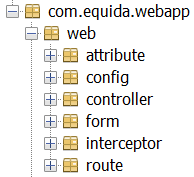
\includegraphics[width=0.33\textwidth, keepaspectratio]{res/webapp-package.png}
				\caption{Packages de WebApp}
			\end{figure}

			\begin{description}
				\item[attribute :]{Contient la classe InputOutputAttribute qui gère toutes les constantes dont on pourrait avoir besoin}
				\item[config :]{Contient les classes relatives à la configuration et la sécurité de l'application}
				\item[controller :]{Contient tous les contrôleurs qui héritent de la classe AbstractWebController}
				\item[form :]{Contient tous les formulaires qui héritent de la classe IForm}
				\item[interceptor :]{Contient la classe UserInterceptor qui hérite de HandlerInterceptorAdapter (voir \nameref{subsec:interceptor} et/ou \href{https://www.tutorialspoint.com/spring_boot/spring_boot_interceptor.htm}{là})}
				\item[route :]{Contient toutes les routes qui héritent de IRoute}
			\end{description}

		\newpage
		\subsection{Resources}

			L'organisation des ressources se présente comme suit :

			\begin{figure}[H]
				\centering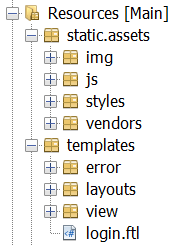
\includegraphics[width=0.23\textwidth, keepaspectratio]{res/ressources.png}
				\caption{Ressources de WebApp}
			\end{figure}

			\begin{description}
				\item[static.assets :]{Contient toutes les ressources statiques qui ne nécessitent aucune compilation}
				\begin{description}
					\item[img :]{Contient toutes les images de l'application}
					\item[js :]{Contient tous les fichiers JavaScript notamment celui pour la gestion des classements à une course d'un cheval et celui pour la page d'accueil avec son carrousel et son menu}
					\item[styles :]{Contient le fichier css de base}
					\item[vendors :]{Contient toutes les dépendances externes du projet soit : Materialize (librairie qui gère le design des vues de l'application), jQuery, Google (police de caractères)}
				\end{description}

				\item[templates :]{Contient tous les fichiers Freemarker}
				\begin{description}
					\item[error :]{Contient les fichiers ftl pour les erreurs 403, 404, 500}
					\item[layouts :]{Contient les fichiers ftl communs à toutes les pages de l'application}
					\item[view :]{Contient toutes les vues de l'applications (lister, consulter, form)}
					\item[login.ftl :]{Fichier utilisé par SpringSecurity pour la page d'authentification}
				\end{description}
			\end{description}

	\newpage
	\section{Configuration de l'application}

		\subsection{application.properties}

			L'application web possède un fichier \textit{application.properties} qui permet de configurer certaines parties de l'application.

			\begin{figure}[H]
				\centering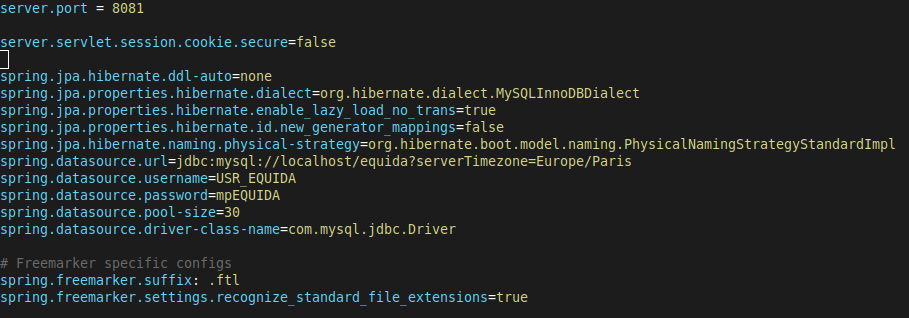
\includegraphics[width=0.85\textwidth, keepaspectratio]{res/application-properties.png}
				\caption{Configuration par application.properties}
			\end{figure}

			Ce fichier configure les informations relatives à l'application dans sa globalité, comme le port à utiliser, la configuration pour connexion avec la \bdd{} (nom utilisateur, mot de passe, ip, ...) ou encore la configuration du moteur de template, FreeMarker en l'occurence.

		\newpage
		\subsection{Configuration par le code}
			\label{subsec:webapp_configCode}

			La configuration de Spring Security est directement faite dans le code source grace à l'utilisation de l'annotation \textit{@Configuration}.

			\begin{figure}[H]
				\centering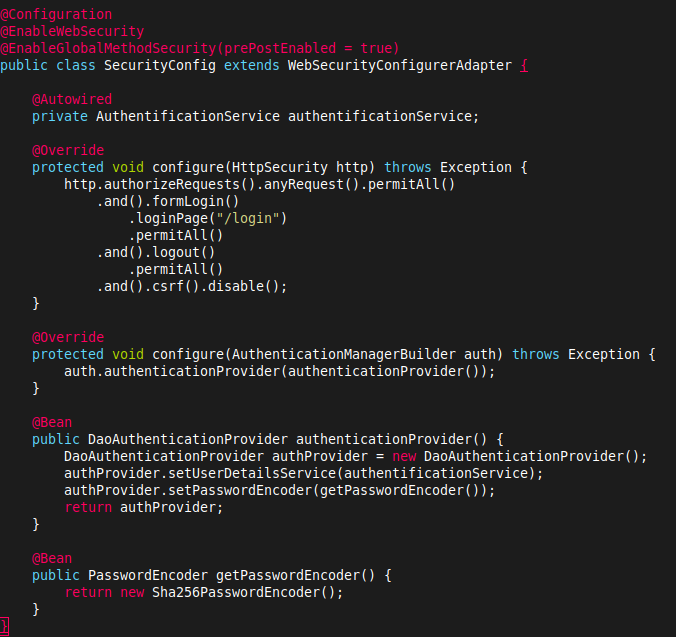
\includegraphics[width=0.75\textwidth, keepaspectratio]{res/SecurityConfig.png}
				\caption{Configuration de Spring Security}
			\end{figure}

			La méthode \textit{void configure(HttpSecurity http)} permet de configurer l'accès aux différentes pages et de changer la configuration des requêtes HTTP. Ainsi, on autorise la connexion sur toutes les pages web, d'autant plus sur login et logout. De cette manière, le jour où l'on décidera de changer cette configuration, le code pour autoriser l'accès à \textit{/logout} et \textit{/login} sera déjà présent et empêchera un potentiel oubli.

			\noindent
			Les méthodes suivantes sont relatives à l'authentification. La méthode \textit{void configure(AuthenticationManagerBuilder)} permet de changer la méthode d'authentification utilisée par Spring Security. Elle fait appel à \textit{DaoAuthenticationProvider authenticationProvider()} qui retourne le DAO à utiliser. On doit donc fournir le \textit{UserDetailsService} du module core, c'est à dire \textit{AuthentificationService} (cf : \nameref{sec:core_authentification}), et le \textit{PasswordEncoder} approprié. De ce fait on utilise donc une nouvelle instance de \textit{Sha256PasswordEncoder} (cf : \nameref{subsec:Sha256PasswordEncoder}).

	\newpage
	\section{Fichiers ressources}

		\subsection{FreeMarker}

			FreeMarker est un moteur de template basé sur Java qui est à l'origine de la génération de pages web dynamiques dans une architecture logicielle.\newline
			Comme mentionné auparavant, tous les fichiers de FreeMarker sont contenus dans le dossier \textit{/resources/templates}. Il est donc possible d'utiliser les directives propres à ce moteur de template.


			\subsubsection{Page de base}

				La page \textit{base.ftl} correspond à la page type de l'application. On y retrouve ainsi ce qui sera inclus sur toutes les pages de l'application. \newline
				Ainsi, \textit{base.ftl} contient le header de la page avec l'inclusion de la feuille de style ; sa partie body contient, elle, le contenu du fichier \textit{nav.ftl} correspondant au menu, ainsi que le footer et les fichiers de scripts nécessaires.\newline
				Les macros permettent le chargement du contenu aux endroits prévus à cet effet. Par exemple, la directive \textit{<@content/>}, présente dans le body de \textit{base.ftl}, chargera le code dans la macro \textit{content} du fichier x.ftl à cet endroit.

				\begin{figure}[H]
					\centering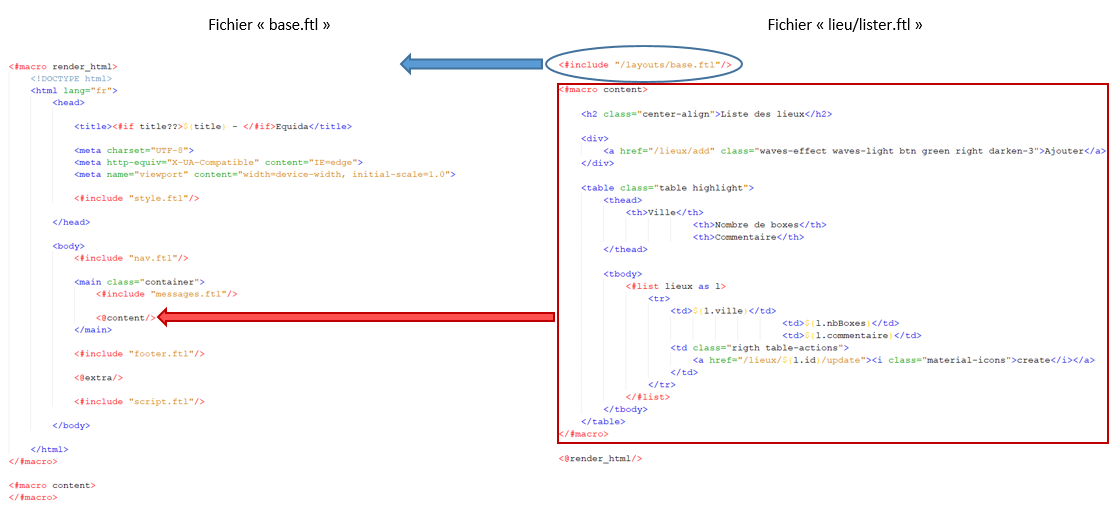
\includegraphics[width=1\textwidth, keepaspectratio]{res/fonctionnementBaseFtl.png}
					\caption{Exemple du fonctionnement de la page base.ftl avec la page lieux/lister.ftl}
				\end{figure}

				\begin{figure}[H]
					\centering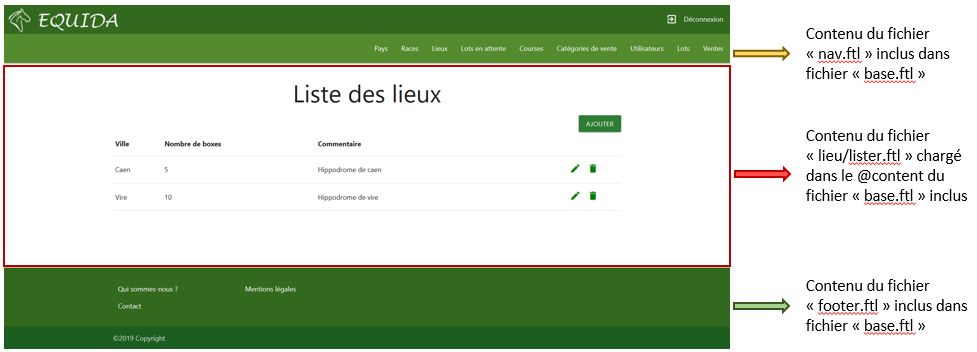
\includegraphics[width=1\textwidth, keepaspectratio]{res/exempleFonctionnementBaseLieuFtl.png}
					\caption{Rendu lors du chargement de la vue qui liste les lieux (correspondant à la page lieux/lister.ftl précédente)}
				\end{figure}

			\subsubsection{Page d'erreur}

				Les pages d'erreur sont chargées automatiquement par Spring et contiennent des messages explicites. Nous avons gérés les erreurs 403 (permissions non autorisées), 404 (page inexistante) et 500 (exception lors de l'exécution du code). Elles reprennent, elles aussi, le design de base de l'application (base.ftl).

				\begin{figure}[H]
					\centering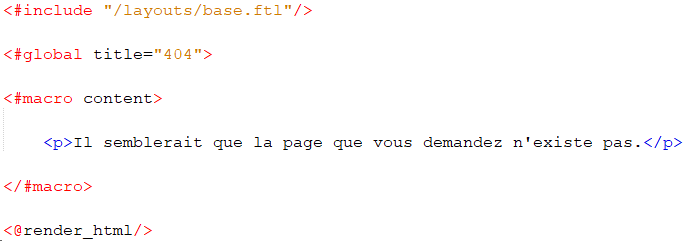
\includegraphics[width=0.75\textwidth, keepaspectratio]{res/codeErreur404.png}
					\caption{Code de l'erreur 404}
				\end{figure}

				\begin{figure}[H]
					\centering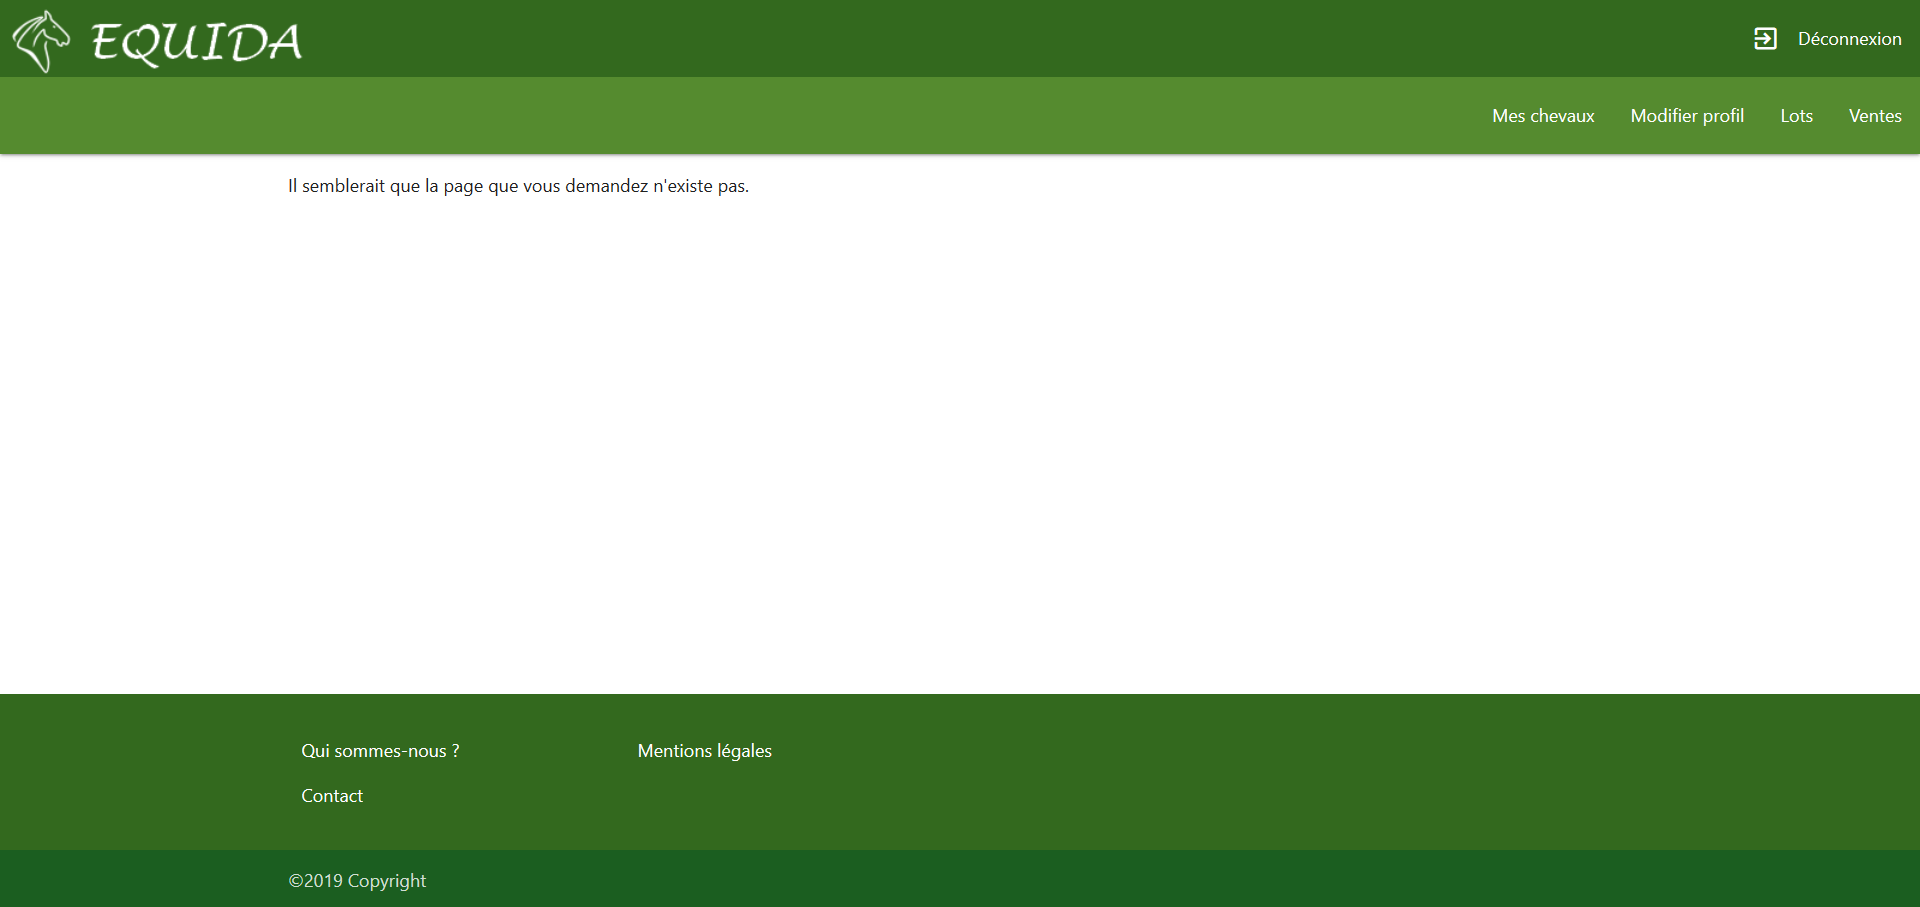
\includegraphics[width=0.85\textwidth, keepaspectratio]{res/exempleErreur404.png}
					\caption{Rendu lors d'une tentative de chargement d'une page inexistante}
				\end{figure}

			\subsubsection{Fichiers à inclure}

				Le dossier \textit{/view/include} contient les vues communes aux différentes pages. On peut les inclure en utilisant les directives \textit{<\#include />}. On retrouve par exemple le fichier \textit{lotLister} qui permet d'afficher les cartes pour les différents lots.

				\begin{figure}[H]
					\centering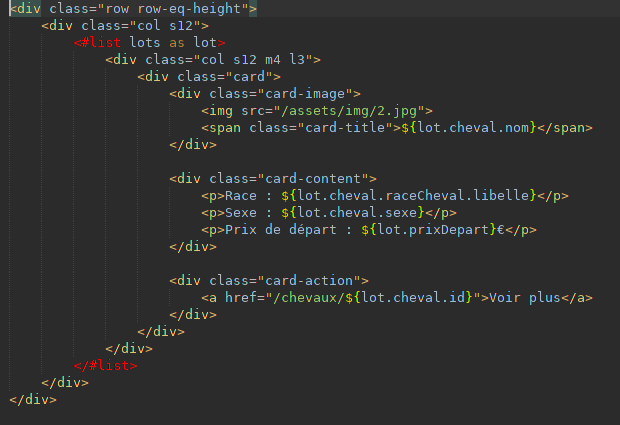
\includegraphics[width=0.75\textwidth, keepaspectratio]{res/include-lotLister.png}
					\caption{Extrait de code du fichier lotLister}
				\end{figure}

				Le code reste celui de n'importe quelle autre vue et ne comporte aucune spécificité.

			\subsubsection{Exemple de page web}

				Ainsi, avec tous les éléments cités précédemment, on peut créer des vues telles que celle ci :

				\begin{figure}[H]
					\centering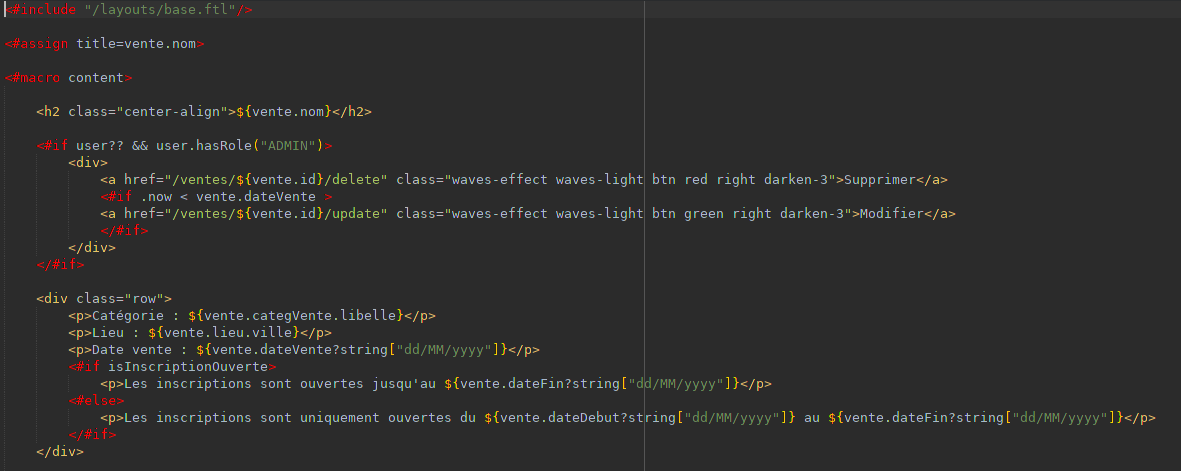
\includegraphics[width=0.85\textwidth, keepaspectratio]{res/view-venteConsulter.png}
					\caption{Code de la vue pour la consultation d'une vente}
				\end{figure}
				On retrouve donc, l'include de \textit{/layouts/base.ftl} pour reprendre le template de base, un changement de valeur concernant le titre, l'utilisation de la macro content, ...

	\section{Gestion de l'authentification}

		\subsection{Gestion template et controller}

			Un contrôleur existe afin de gérer l'affichage d'un template FreeMarker concernant la page de connexion à l'application. Ce contrôleur se charge uniquement de l'affichage de l'information. En effet, le traitement des identifiants est fait par Spring Security (comme mentionné dans \nameref{subsec:webapp_configCode}).

		\subsection{Interceptor}
			\label{subsec:interceptor}

			Afin de faciliter la gestion de l'utilisateur actuellement connecté dans la vue ou les contrôleurs, une classe \textit{UserInterceptor} permet de fournir automatiquement l'instance de \textit{AuthentificatedUser} à la vue ou au contrôleur.

			\begin{figure}[H]
				\centering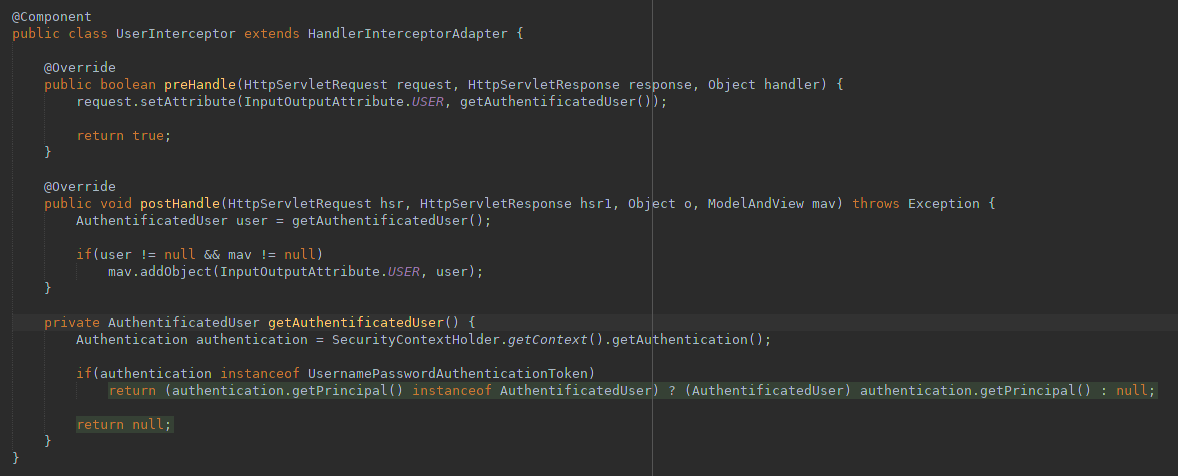
\includegraphics[width=0.85\textwidth, keepaspectratio]{res/UserInterceptor.png}
				\caption{Code de UserInterceptor}
			\end{figure}

			\noindent
			On peut alors avoir accès à la variable \textit{user} dans la vue comme n'importe quelle variable fournie par le contrôleur ou dans le contrôleur en utilisant le paramètre suivant dans une méthode d'un controleur \textit{@RequestAttribute(name = InputOutputAttribute.USER, required = false) AuthentificatedUser user}.

	\section{Exemple Route}

		L'interface \textit{IRoute} décrit les méthodes qui doivent être implémentées par les classes filles.\newline
		Ainsi chaque fichier route contiendra une méthode \textit{getUri()}, une méthode \textit{getView()} et \textit{getTitle()} qui retourneront respectivement l'URL, la vue et le titre à utiliser dans la page concernée (pour la route correspondante).

		\noindent
		Par exemple, pour \textit{PaysRoute}, qui est donc la route principale selon notre nomenclature, l'URL correspond à \textit{/pays}, c'est à cette url là, qu'on chargera la vue \textit{pays/lister} avec le titre "Les pays".

		\begin{figure}[H]
			\centering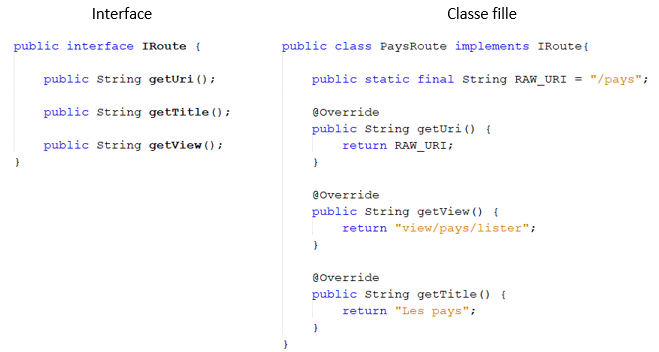
\includegraphics[width=0.75\textwidth, keepaspectratio]{res/paysRoute.png}
			\caption{Code de l'interface et utilisation par la classe fille PaysRoute}
		\end{figure}

		\begin{figure}[H]
			\centering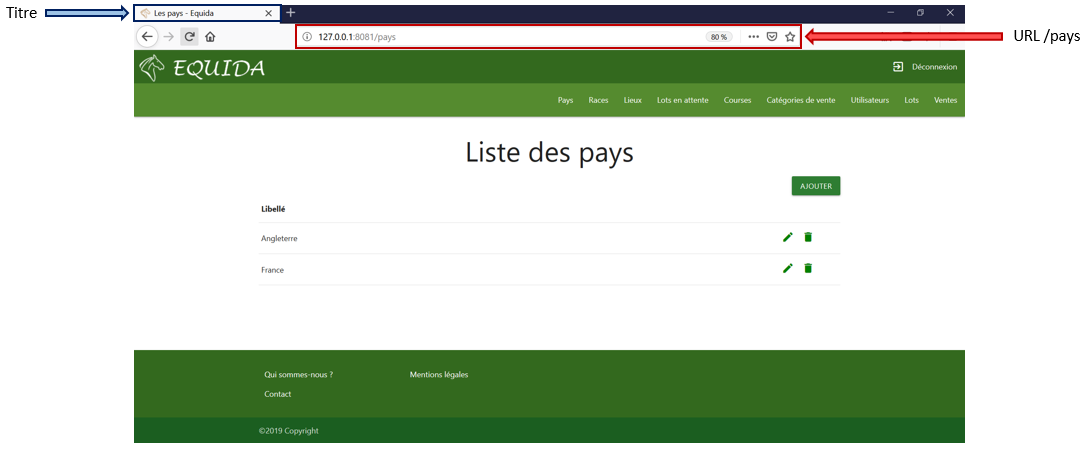
\includegraphics[width=0.85\textwidth, keepaspectratio]{res/renduPaysRoute.png}
			\caption{Rendu obtenu avec la vue pays/lister}
		\end{figure}

	\section{Exemple Form}

		La classe mère \textit{IForm} est une classe abstraite qui utilise la générécité ce qui nous permettra d'adapter les méthodes en fonction de l'entité x pour laquelle le formulaire est fait. L'héritage nous permet donc d'utiliser les variables et méthodes déclarées dans le formulaire neutre xForm.\newline
		Par exemple, prenons l'entité \textit{Lieu}. On crée le formulaire "neutre" \textit{LieuxForm} qui héritera de \textit{IForm} et qui permettra de définir les éléments communs aux formulaire d'ajout et de modification.\newline
		On fera donc hériter de ce formulaire "neutre" \textit{LieuxAddForm} et \textit{LieuxUpdateForm} et on passera, dans un premier cas, le la variable \textit{isCreation} à true et dans le second, à false.

		\begin{figure}[H]
			\centering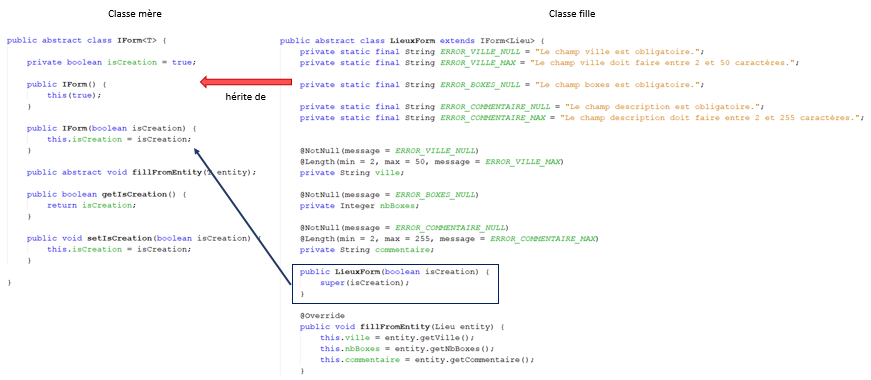
\includegraphics[width=1\textwidth, keepaspectratio]{res/IForm.png}
			\caption{Exemple implémentation interface IForm avec LieuxForm}
		\end{figure}

		\begin{figure}[H]
			\centering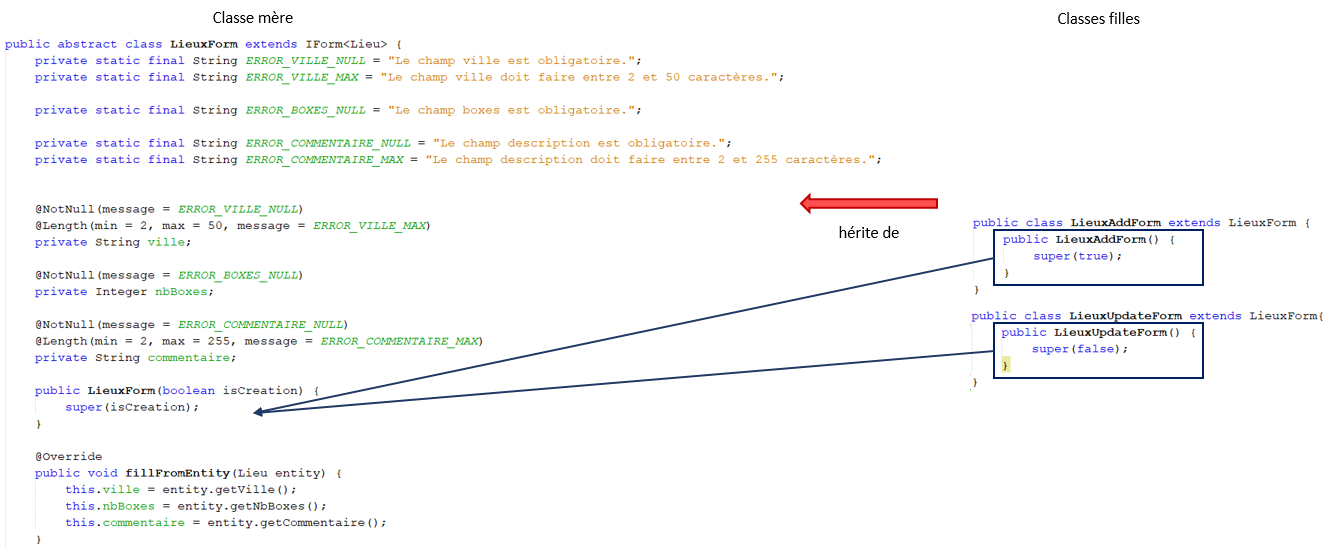
\includegraphics[width=1\textwidth, keepaspectratio]{res/formClassFilles.png}
			\caption{Exemple avec LieuxUpdateForm et LieuxAddForm}
		\end{figure}

	\newpage
	\section{Classe InputOutputAttribute}

		Cette classe permet la définition de constantes qui seront utilisées au travers de l'application.

		\begin{figure}[H]
			\centering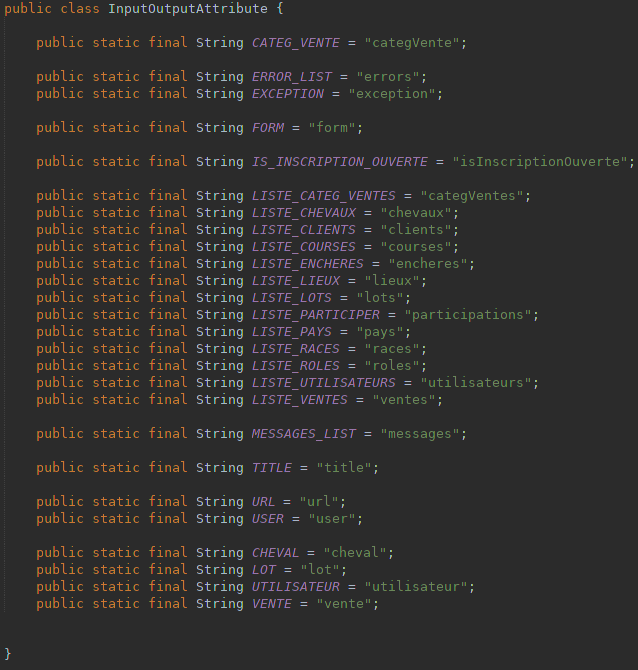
\includegraphics[width=0.75\textwidth, keepaspectratio]{res/InputOutputAttribute.png}
			\caption{Code de InputOutputAttribute}
		\end{figure}

		Ces constantes permettent de garder une unité dans la définition des noms et d'éviter d'éventuelles erreurs d'écriture. Ainsi, lorsque l'on doit fournir une clé de type String on pourra utiliser une des constantes de la classe. Elles sont donc très utilisées pour transmettre les informations du contrôleur vers la vue.

		\begin{figure}[H]
			\centering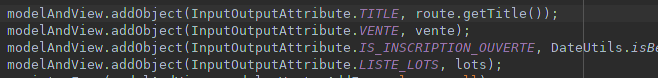
\includegraphics[width=0.75\textwidth, keepaspectratio]{res/InputOutputAttribute-controller.png}
			\caption{Exemple d'utilisation de InputOutputAttribute}
		\end{figure}

	\newpage
	\section{Les Contrôleurs}

		\subsection{AbstractWebController}

			Cette classe est la classe mère de tous les contrôleurs. On y définit certaines méthodes, par exemple, la possibilité d'ajouter des messages d'erreurs, qui seront transférées à la vue.

			\begin{figure}[H]
				\centering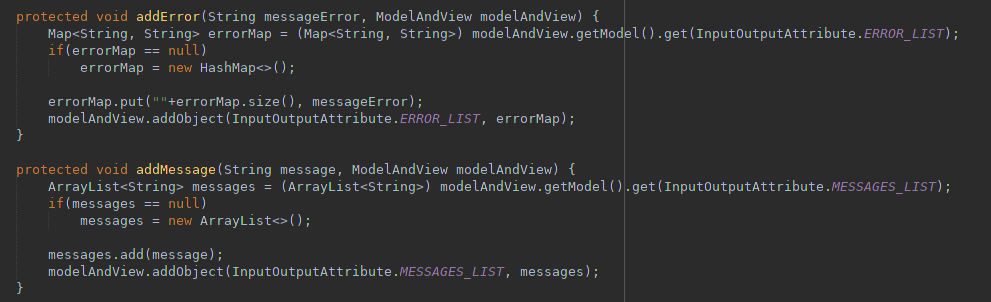
\includegraphics[width=0.85\textwidth, keepaspectratio]{res/AbstractWebController-messages.png}
				\caption{Méthodes pour la gestion des messages}
			\end{figure}

			\noindent
			On y implémente aussi la gestion des exceptions, dans lesquelles, on passe les variables nécessaires au bon affichage de la vue.

			\begin{figure}[H]
				\centering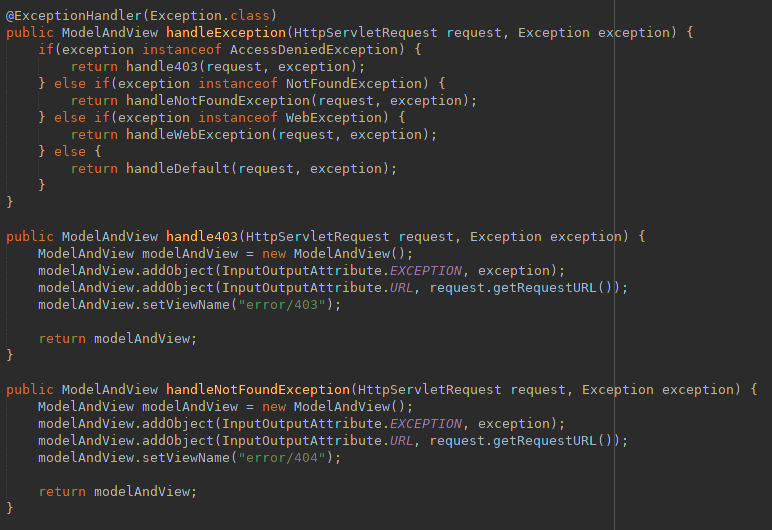
\includegraphics[width=0.75\textwidth, keepaspectratio]{res/AbstractWebController-exception.png}
				\caption{Méthodes pour la gestion des exceptions}
			\end{figure}

			\newpage
			\noindent
			Elle comprend, en plus, 2 méthodes qui permettent de simplifier le code de gestion des formulaires, l'une afin de les créer et de les compléter si besoin, l'autre afin de faciliter la gestion des erreurs sur ceux-ci.

			\begin{figure}[H]
				\centering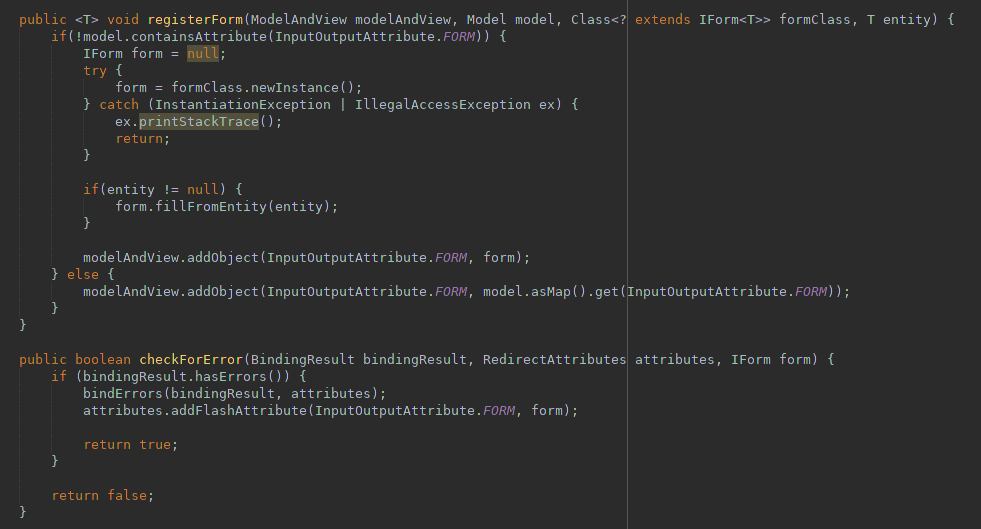
\includegraphics[width=0.80\textwidth, keepaspectratio]{res/AbstractWebController-form.png}
				\caption{Méthodes pour la gestion des formulaires}
			\end{figure}

		\subsection{Exemple Controller}

		Les différents contrôleurs créés pour les entités x héritent tous de la classe AbstractWebController. \newline
		Les contrôleurs contiennent différentes méthodes associées aux méthodes GET, POST, PATCH et DELETE ainsi qu'a une route. Enfin, elles utilisent les services pour intéragir avec la \bdd{}. On y définit aussi les différentes autorisations avec l'annotation @PreAuthorize afin de savoir qui peut accéder à la page, et donc, executer la méthode.

		\noindent
		Par exemple, dans \textit{EncheresController}, la méthode \textit{addGet} n'est possible que pour un utilisateur ayant le role 'ADMIN', elle est reliée à l'URL \textit{EncheresAddRoute.RAW\_URI} (URL stockée dans la variable constante RAW\_URI de la classe \textit{EncheresAddRoute}). Elle permet de récupérer les différentes variables nécessaires à l'affichage de la page, comme le formulaire d'ajout d'une enchère par exemple.

		\begin{figure}[H]
			\centering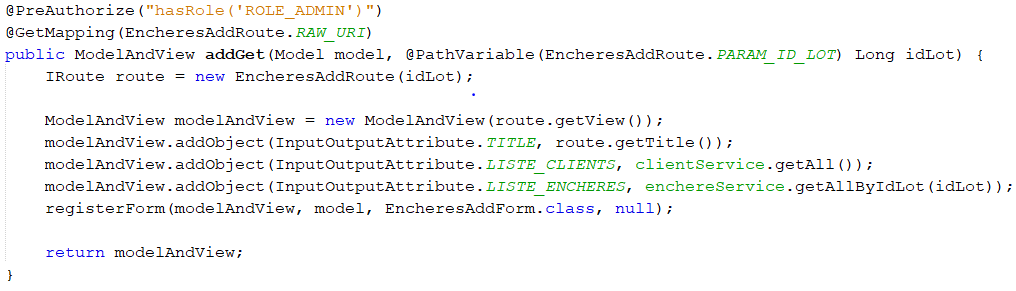
\includegraphics[width=0.95\textwidth, keepaspectratio]{res/enchereController.png}
			\caption{Exemple d'un contrôleur}
		\end{figure}
